\chapter{Deep learning neural networks}
\label{chap:deep}
\section{Context}
Deep learning neural networks gained popularity again in recent years, after the AI winter ended. Since then neural networks became part of the everyday life, we hear about artificial intelligence being used in smart phones to enhance images quality or recognize certain settings and take a picture accordingly. AI is also being used in cancer research and other fields of bioinformatics, and personal assistants became extremely popular.

But even with the seemingly endless capabilities of artificial neural networks we are far from creating anything that could pass the Turing test, let alone have the cognitive capacities of humans. This problem is AI-complete or AI-hard, meaning that creating a network that could keep up a human-like conversation would require data scientist and researchers to construct a universal artificial intelligence. A small but important step to achieve this is to create a system capable of doing simple reading comprehension tasks that also require some common sense knowledge.

The most common structures of these experimental neural networks include recurrent neural network layers and attention layers. Before we explain the function of these building-blocks we need to lay down a foundation.

\section{Basics}
Artificial neural networks are said to mimic the human neural networks, which is true on the surface, but mathematically speaking they are more like a complex mathematical functions that tries to predict an output with the given set of inputs.
\subsection{Perceptron}
Perceptrons are the binary linear classifying units of the neural network. They function like neurons (Figure~\ref{fig:neuron}) so to speak.
\begin{figure*}[!htb]
	\centering
	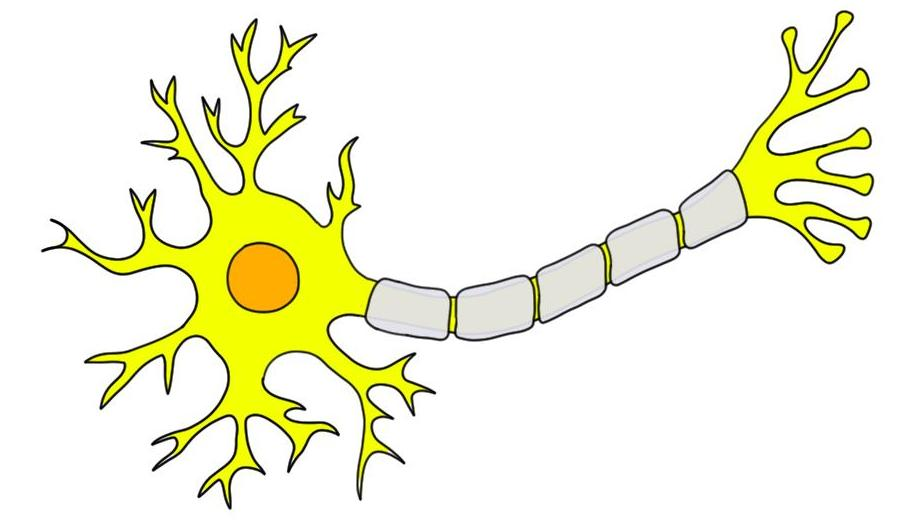
\includegraphics[scale=0.1]{neuron.jpg}
	\caption{Neurons are usually depicted like this. Image from the \textit{Neuroscientifically Challenged} website.}
	\label{fig:neuron}
\end{figure*}
Neurons fire if certain dendrites receive signals. Similarly, a perceptron "fires" if its input vector's weighted sum is above a certain bias.
\[output = \sum (input * weight) + bias\]
But what are these parameters?

The weight could be loosely explained like the strength of a given input, how much should it affect the output value. Bias is a threshold we set for the perceptron.
\subsection{Feed forward}
The layers of the neural network consist of these perceptrons. A simple structure is depicted in Figure~\ref{fig:neural_net}.
\begin{figure*}[!htb]
	\centering
	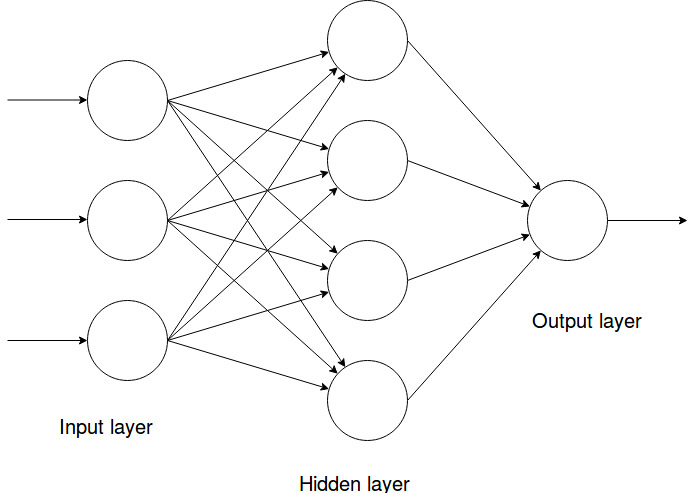
\includegraphics[scale=0.5]{simple_neural_network.jpg}
	\caption{A simple feed forward neural network.}
	\label{fig:neural_net}
\end{figure*}

This neural network consists of feed-forward layers, which means that every perceptron in each layer connects to every perceptron in the previous and the next layer. Each connection has a weight value attached to it. The output of this network is constructed as follows:
\[output = \sum activationFunction(\sum(input * weight_1 + bias_1)) * weight_2 + bias_2\]
Here the activation function is a function that the hidden layer's output passes through. It is used to add non-linearity to the network. This will be crucial in the backpropagation step.
There are multiple types of activation functions in deep learning, the most commons being tanh (Figure~\ref{fig:tanh}), sigmoid (Figure~\ref{fig:sigmoid}), relu and its variations.
\[tanh(x) = \frac{e^x - e^{-x}}{e^x + e^{-x}}\]
\begin{figure*}[!htb]
	\centering
	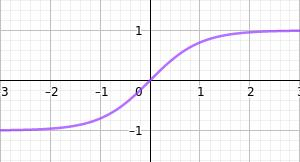
\includegraphics[scale=0.5]{tanh.jpg}
	\caption{Hyperbolic tangent activation function}
	\label{fig:tanh}
\end{figure*}
\[sigmoid(x) = \sigma(x) = \frac{1}{1 + e^{-x}}\]
\begin{figure*}[!htb]
	\centering
	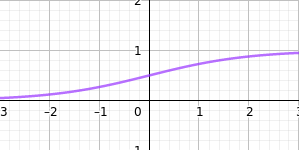
\includegraphics[scale=0.5]{sigmoid.jpg}
	\caption{Sigmoid activation function}
	\label{fig:sigmoid}
\end{figure*}
\[relu(x) = \begin{cases}x & \quad \text{if } x \geq 0 \\ 0 & \quad \text{else}\end{cases}\]
\begin{figure*}[!htb]
	\centering
	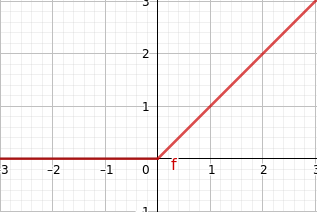
\includegraphics[scale=0.5]{relu.jpg}
	\caption{Rectified linear unit activation function}
	\label{fig:relu}
\end{figure*}
\subsection{Backpropagation}
In the Feed forward section we mentioned the bias and weight parameters. In this section we will describe the method of fine tuning these parameters so the neural network will be better at prediction.
To do this we will need to first calculate the loss of the network. This means that we compare expected output and the calculated output (we can do this because we are doing supervised learning). There are multiple types of loss functions like squared loss used at regression problems and cross entropy at classification problems. Right now we will need the later which we can get by taking the negative natural logarithm of the \(P(output|layerInput, parameters)\) probability.
Let's use the following notation :

\(output = y\)

\(output's \text{ i}th \text{ } value = y_i\)

\(layerInput = x\)

\(layerInput's \text{ i}th \text{ } value = x_i\)

\(activationFunction = \sigma\)

\(parameters = w\)

And the parameters are the vector of the weights concatenated with the bias.
The negative natural logarithm of \(P(output|layerInput, parameters)\) is:
\[Loss = -\ln P(y|x, w) = \sum_{i=1}^{|classes|}y_i\ln \sigma(w^Tx_i)+(1 - y_i)\ln (1 - \sigma(w^Tx_i))\]
In a simple two class classification where we only have one output (0 or 1) it simplifies to:
\[Loss = -\ln P(y|x, w) = y_i\ln \sigma(w^Tx_i)+(1 - y_i)\ln (1 - \sigma(w^Tx_i))\]
After we calculated this, we are ready for the error backpropagation. Let's calculate the gradient of this Loss by the parameters.
\[\Delta_w Loss = -\sum_{i=1}^{|classes|}(y_i - \sigma(w^Tx_i))x_i\]
Now all we have to do is to use this n every layer backwards.
\[\Delta_x Loss = \sum_{k} \frac{\delta Loss}{\delta w^k}\frac{\delta w^k}{\delta x}\]
\[\frac{\delta w^k}{\delta x} = \sigma'(activated)*previousLayer\]
where:
\[activated = \sigma(x * previousLayer)\]
Once we calculated this delta for every layer, all we have left to do is to update the parameters.
\[w \leftarrow w - \eta * \Delta_x Loss\]

Where \(\eta\) is the learning rate, that we can set. This an important parameter, because if we set it too low, our network will learn really slowly, and it will probably stuck in a local minimum. But setting it too high has its dangers too, since we can jump over the global optimum and the network will never stabilize.

\subsubsection{Optimization}
The goal of optimization is to overcome the following problems:
\begin{itemize}
	\item Local minimum
	\item Setting the learning rate
	\item Setting the batch size
\end{itemize}

We have touched on the first two briefly before, but setting the batch size is also very important. We give the training data to the network in batch-es, and we iterate through them multiple times (depending on the epoch). The loops length is the number of epochs we take.

Methods used for optimizing:
\begin{itemize}
	\item \textbf{Stochastic gradient descent}
	\item \textbf{Momentum}
	\item \textbf{Adaptive learning rate}
	\item \textbf{Adam} (Adaptive learning rate and momentum)
\end{itemize}

\paragraph*{Stochastic gradient descent}
\[g \leftarrow \frac{1}{batchSize}\Delta_w \sum_{i=1}^{batchSize}Loss(\Phi_w(x_i), y_i)\]
Where \(\Phi\) is the network itself.
\[w \leftarrow w - \eta g\]

\paragraph*{Momentum}
\[g \leftarrow \alpha g + \frac{1}{batchSize}\Delta_w \sum_{i=1}^{batchSize}Loss(\Phi_w(x_i), y_i)\]
Where \(\alpha\) is a parameter we can set.
\[w \leftarrow w - \eta g\]

\paragraph*{Adaptive learning rate}
\[g \leftarrow \frac{1}{batchSize}\Delta_w \sum_{i=1}^{batchSize}Loss(\Phi_w(x_i), y_i)\]
\[r \leftarrow r + g^2\]
Where r is a parameter thats initial value can be set.
\[w \leftarrow w - \frac{\eta}{\sqrt{r}} g\]

\paragraph*{Adam}
\[g \leftarrow \frac{1}{batchSize}\Delta_w \sum_{i=1}^{batchSize}Loss(\Phi_w(x_i), y_i)\]
\[r \leftarrow \varphi_r r + (1 - \varphi_r) g^2\]
\[s \leftarrow \varphi_s s + (1 - \varphi_s) g\]
Where s is a parameter thats initial value can be set and \(\varphi\) is a parameter.
\[w \leftarrow w - \frac{\eta s}{\sqrt{r}} g\]

\subsubsection{Regularization}
The goal of regularization is to avoid over-fitting. Over-fitting happens when our neural network produces good results on the training set's dedicated subset, the development or validation set, but it can't predict the expected outputs properly on a new dataset for example the test set. It happens very often, so machine learning experts developed a couple functions to avoid this phenomenon.
\begin{itemize}
	\item \textbf{Weight decay}: It uses a parameter to make sure that the previously learned weight won't influence the new one too much. \(w \leftarrow (1 - \eta \alpha)w - \eta \Delta_w Loss\)
	\item \textbf{Dropout}: It randomly "drops out" weights for an epoch, so they won't over-fit
	\item \textbf{Early stopping}: It stops the learning if the results on the development set haven't shown any progress in the last couple of epochs.
	\item \textbf{Noise injection}: It injects noise into the training set.
\end{itemize}

\section{Natural Language Processing with Deep learning}
As mentioned above the kind of layers used in Natural Language Processing are mostly recurrent neural network layers and attention layers.
\subsection{Recurrent Neural Networks}
In a simple feed forward neural network, the information only moves in one direction: from the input layer to the output layer. On the other hand recurrent neural networks have a so called short term memory. This internal memory allows the network to "remember" what it had learned before. This is illustrated at Figure~\ref{fig:recurrent_net}.
\begin{figure*}[!htb]
	\centering
	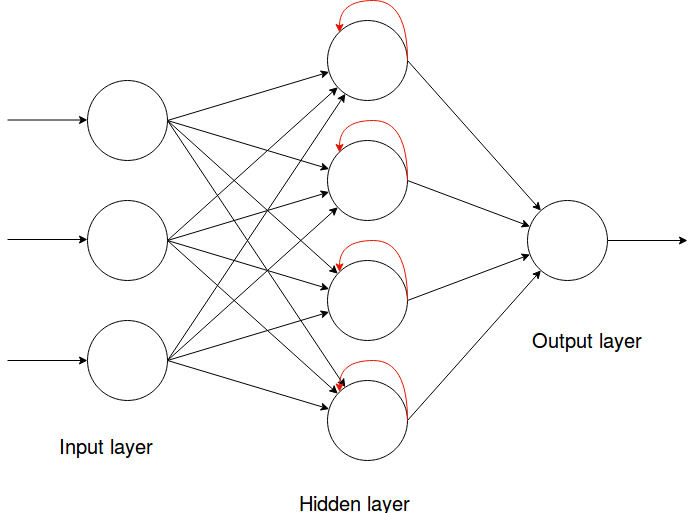
\includegraphics[scale=0.5]{recurrent_neural_network.jpg}
	\caption{A recurrent neural network.}
	\label{fig:recurrent_net}
\end{figure*}

The backpropagation is also slightly different in this case, it's called backpropagation through time, you need to "unroll" the network (see at Figure~\ref{fig:unrolled}), and use the backpropagation starting from the right timestamps. Each timestamp's backpropagation could be understood as backpropagation on a separate feed forward neural network. 
\begin{figure*}[!htb]
	\centering
	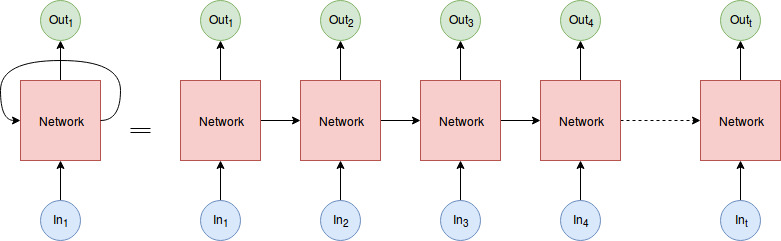
\includegraphics[scale=0.5]{unrolled.jpg}
	\caption{Unrolled recurrent neural network.}
	\label{fig:unrolled}
\end{figure*}

The gradient vanishing or explosion can be a problem with this RNN.
\subsubsection{Long-Short Term Memory}
Long-short term memory networks ar the extension of the previously discussed recurrent neural network. The main difference is that it also has an internal long term memory. It is implemented with three gates:
\begin{itemize}
	\item \textbf{input gate}: determines whether to let new input in
	\item \textbf{forget gate}: determines whether to forget an input because it's not relevant anymore
	\item \textbf{output gate}: determines whether to let the input impact the output with the current timestamp
\end{itemize}
These gates are analog and their value ranges from 0 to 1 with the sigmoid function. A simplified depiction can be seen at Figure~\ref{fig:lstm}.
\begin{figure*}[!htb]
	\centering
	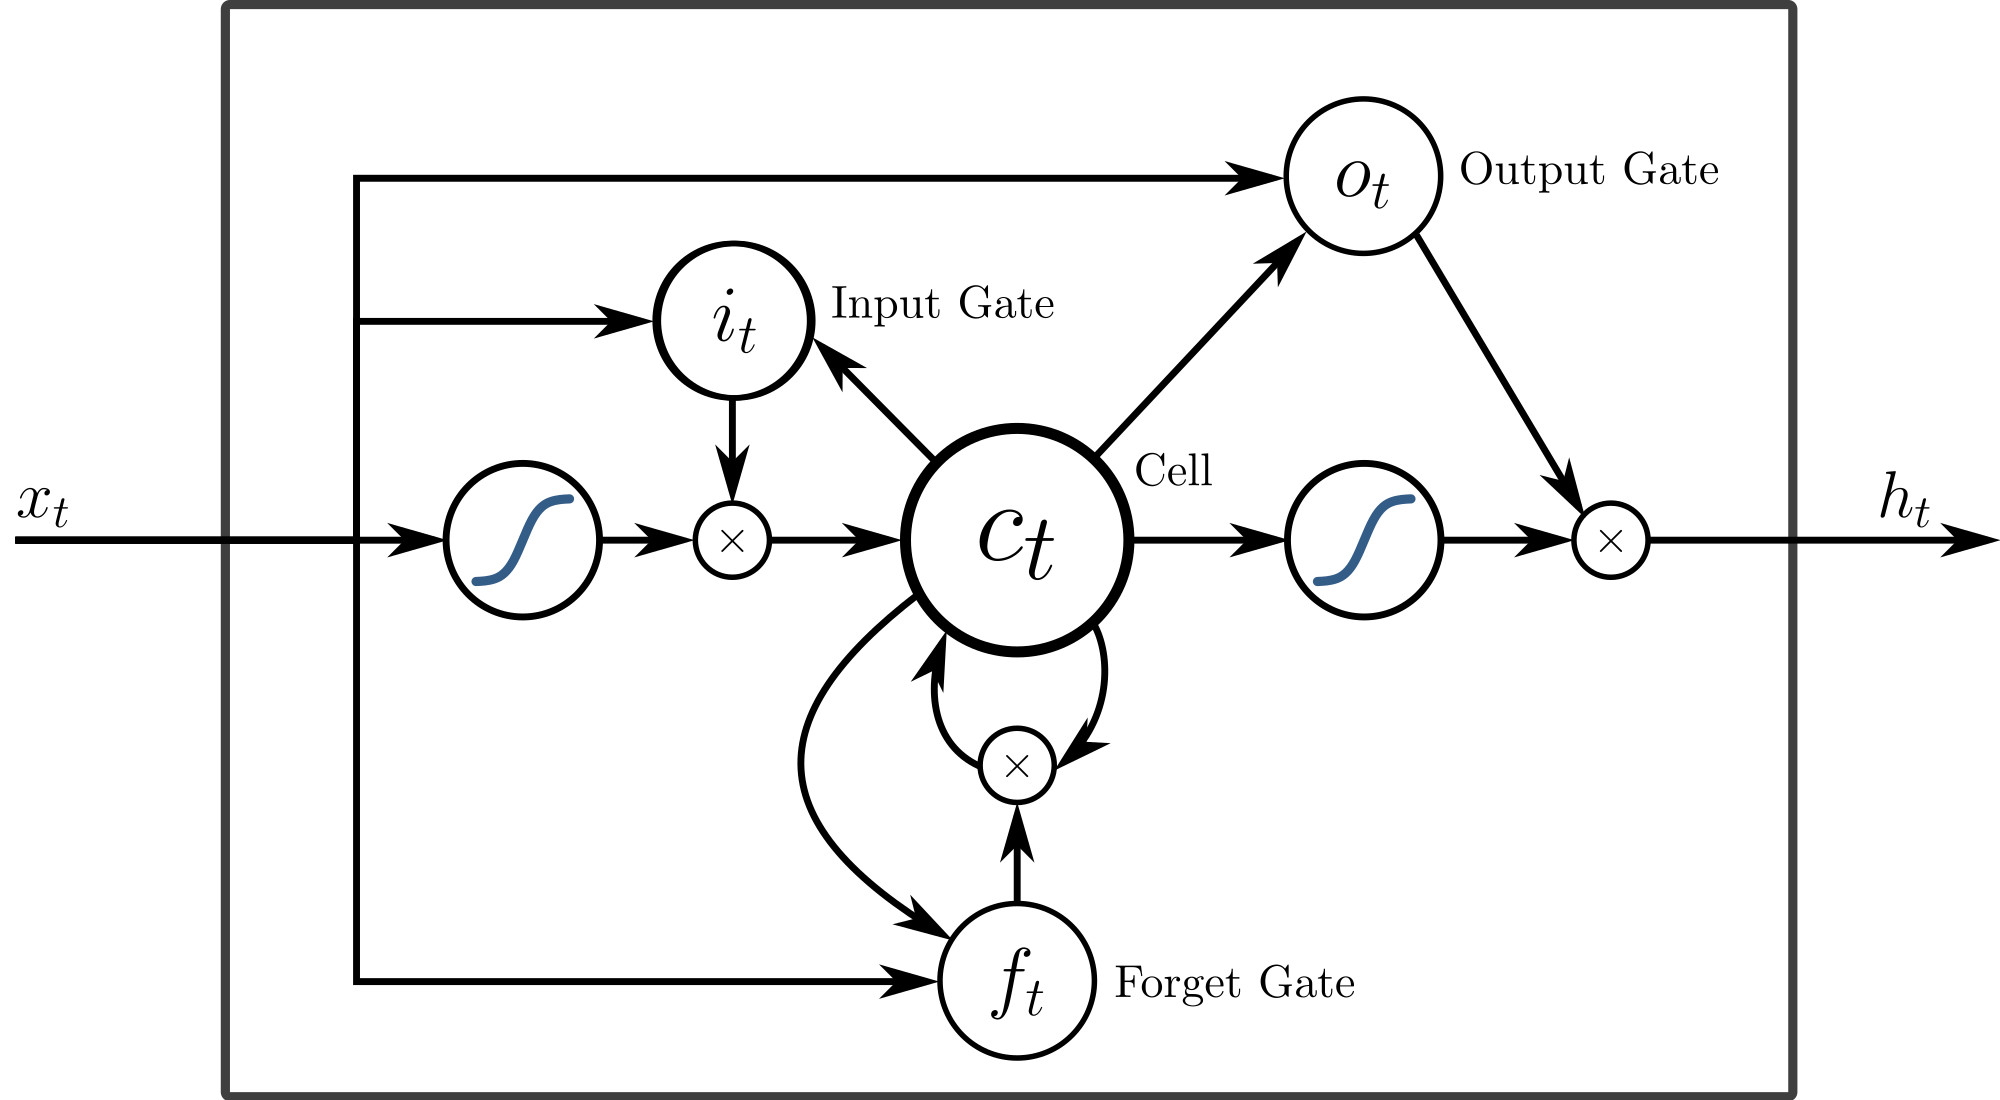
\includegraphics[scale=0.2]{lstm.jpg}
	\caption{A long-short term memory network's gates.\\Image from Wikipedia}
	\label{fig:lstm}
\end{figure*}

The sigmoid function allows this structure to be able to learn, meaning that we can use the backpropagation method described above.

\subsubsection{Gated recurrent unit}
Gated recurrent units are also a type of RNN and have a similar structure (Figure~\ref{fig:gru}) to the long-short term memory network, but has been shown to exhibit better performance on smaller datasets, than the LSTM.
\begin{figure*}[!htb]
	\centering
	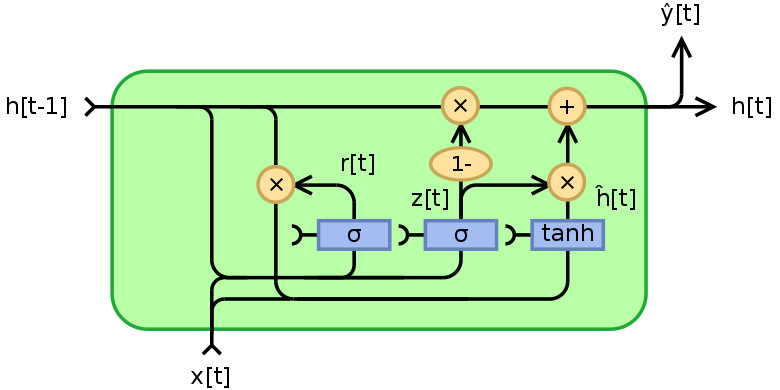
\includegraphics[scale=0.5]{gru.jpg}
	\caption{A gated recurrent unit's gates.\\Image from Wikipedia}
	\label{fig:gru}
\end{figure*}

It has four main building blocks:
\begin{itemize}
	\item \textbf{update gate}: the gate gets the x[t] and the h[t-1] as its input and z[t] is the output on the image
	\item \textbf{reset gate}: the gate gets the x[t] and the h[t-1] as its input and r[t] is the output on the image
	\item \textbf{current memory content}: the gate gets the x[t], the h[t-1] and the r[t] as its input and \^{h}[t] is the output on the image
	\item \textbf{final memory at current time step}: the h[t] on the image
\end{itemize}

Gated recurrent units are mostly used on the field of speech recognition and music modeling while the LSTM is more relevant on the field of natural language processing.

\subsection{Attention}
The Attention mechanism was first described in \cite{Bahdanau:2015} and was used for machine translation. Since then it became a widely used tool in natural language processing. The idea behind this mechanism is that when the neural network predicts the output, it only uses parts of the given input instead of the full input. That is where the most relevant informations are concentrated and this mechanism only pays \textit{attention} to these parts.

Usually in the "sequence-to-sequence" tasks like MT there are two main parts of the model an encoder and a decoder. The encoder is responsible for creating a so called context-vector from the input sequence. This context-vector has a fixed length and it serves as the representation of the sequence inside the model. The decoder then decodes this context-vector to a sequence again, in the case of the machine translation this sequence is in a different language. A depiction can be seen at Figure~\ref{fig:seq_to_seq}.
\begin{figure*}[!htb]
	\centering
	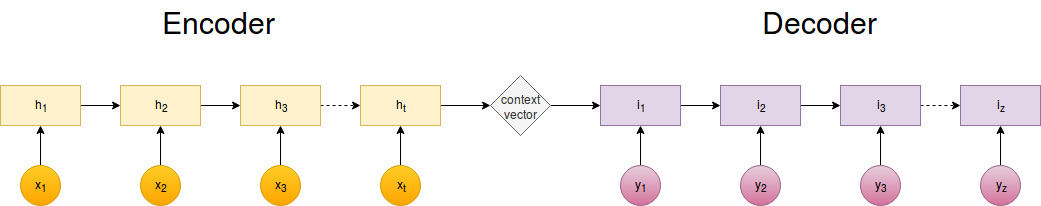
\includegraphics[scale=0.4]{seq_to_seq.jpg}
	\caption{A sequence-to-sequence model with encoder and decoder.}
	\label{fig:seq_to_seq}
\end{figure*}

The attention mechanism described in \cite{Bahdanau:2015} was used in the decoder part of this model, the encoder functions the same way. The paper explicitly stated that this attention mechanism relieves the encoder from having to encode every sequence to a fixed length context vector. In this case we have a context vector for every word of the expected output. These context-vectors are the weighted sums of the encoder's states (\textit{annotations}).
\[c_i = \sum_{j=1}^{t} \alpha_ij h_j\]
Where \(\alpha\) parameter is calculated like the following:
\[\alpha_ij = \frac{exp(e_{ij})}{\sum_{k=1}^{t} e_{ik}} \]
and \(e_{ij}\) is its energy
\[e_{ij} = a(s_{i-i}, h_j)\]
This is an \textit{alignment model} that scores how well the input around \textit{j} and the output around \textit{i} match. This \textit{alignment model} is a feed forward neural network that is trained simultaneously with the other components of the system.
The decoder uses the previous state's output and its assigned context-vector when calculating its own target.
\[s_i = f(s_{i-1}, y_{i-1}, c_i)\]
The attention based model is at Figure~\ref{fig:attention}.
\begin{figure*}[!htb]
	\centering
	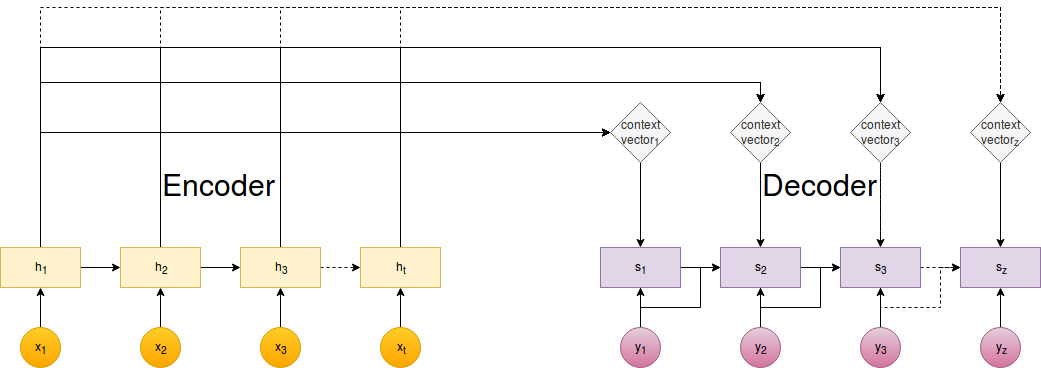
\includegraphics[scale=0.4]{attention.jpg}
	\caption{A sequence-to-sequence model with encoder-decoder and attention.}
	\label{fig:attention}
\end{figure*}

A big advantage of using this mechanism is the ability to interpret our model. These days it's more important than ever to be able to tell why does the network predict what it predicts, and thanks to the attention mechanism we are able to say that (in a purely attention-based network). One example is shown at Figure~\ref{fig:interpretation}.

\begin{figure*}[!htb]
	\centering
	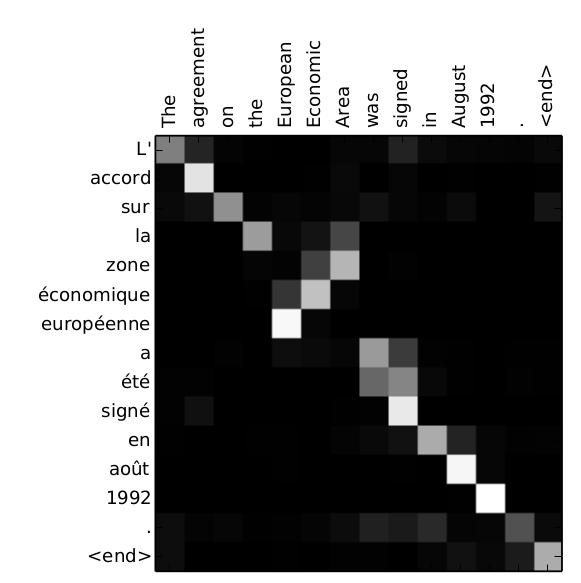
\includegraphics[scale=0.4]{interpretation.jpg}
	\caption{An interpretation of a french to english translation.\\Image from \cite{Bahdanau:2015}.}
	\label{fig:interpretation}
\end{figure*}

\begin{minipage}{\linewidth}
	Since its first description in \cite{Bahdanau:2015} the attention mechanism has been used for:
	\begin{itemize}
		\item \textbf{Image description}: a convolutional neural network translates the image to the context vectors and the decoder creates a description for it.
		\item \textbf{Grammar representation}: in this case the decoder builds a grammatical representation for the input.
		\item \textbf{Machine comprehension tasks}: question answering based on a previously read text. 
	\end{itemize}
\end{minipage}